There are jobs that are trivial for all people, even for kids, but they are extremely difficult even for the most powerful and sophisticated software and software. This type of task has as its characteristics the need for creativity and level of abstraction which, in the present moment, is slightly in the minds of human beings. 

Some examples classify this type of task with image recognition, especially when there is occlusion or involves subjective analysis, content authorship, analysis of emotions and so many other activities that inherently require human intelligence to be performed. Luis von Ahn introduced in his dissertation  \cite{VonAhn:2005:HC:1168246}  a paradigm named Human Computation that allows to approach the problems from this point of view, identifying in it what tasks can be automated and which are those that require human treatment. Additionaly Human Computation can improve performance by division of labor because it helps to define tasks that can be executed in parallel \cite{Rohwer:2010:NHC:1837885.1837897}.

One of the benefits of modeling a system according to the Human Computation paradigm is to focus the effort of human collaborators only on tasks that really require their attention, this is done by identifying the tasks that inherently require human intelligence. Each of these tasks is a HIT (Human Intelligence Task) and corresponds to something that humans can easily solve while a machine presents extreme difficulty in trying to solve \cite{doi:10.2200/S00371ED1V01Y201107AIM013}. 

In short, Human Computation is a paradigm that proposes to identify into the problems which tasks require human intelligence and which tasks can be automated. In general, it may be benefited with modeling based on the Human Computation paradigm the problems in which it is possible to identify tasks that are very difficult for machines but which can be easily completed by humans. In terms complexity, a HIT can be a microtask or a macrotask. These strategy is ilustrated in ~\ref{hc}.

\begin{figure}[ht]
\centering
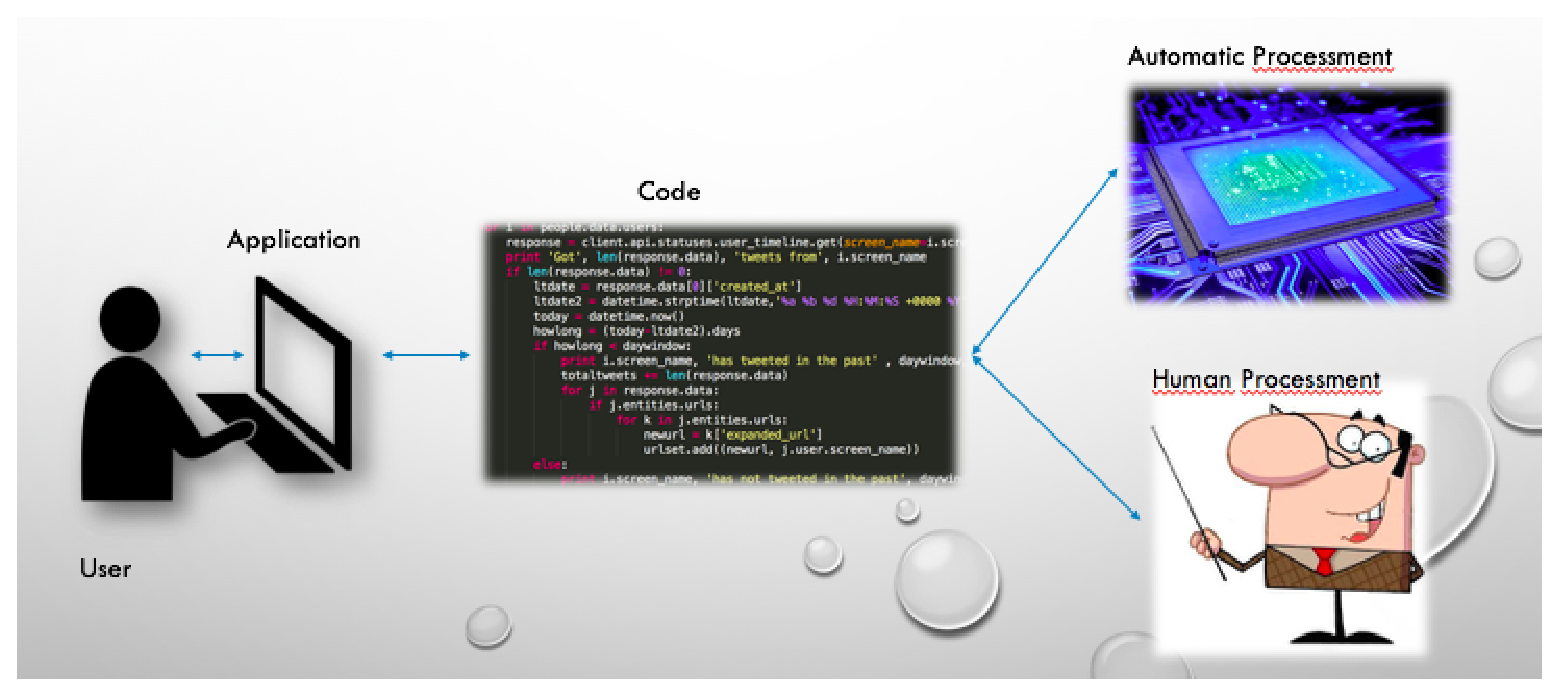
\includegraphics[scale=0.3]{figure/hc}
\caption{Human Computation}
\label{hc}
\end{figure}

Macrotasks require more effort from the worker, often requiring him to be an expert in the field or to have training on subjects related to the task. In the context of media annotation, this type of task is suitable for complex annotations because it assumes that the worker is qualified and will devote the time and effort required to complete it. However, macrotasks often require sophisticated annotation systems and limit the group of workers who are able to execute them \citep{Haas:2015:AMC:2824032.2824062}. In this work, complex annotations are defined as those that combine annotations on different aspects of annotated objects and therefore are usually obtained by macrotasks.

On the other hand, microtasks are usually modeled in a way that can be accomplished quickly and easily by less skilled workers. For media annotation, this kind of task is usually used to generate simple annotations, which refer to one or a few items to be annotated in each task. Also, often a Microtask can be performed using a simple annotation tool. 

Microtasks are widely used in crowdsourcing projects and this kind of task is supported by well-established commercial platforms such as Amazon Mechanical Turk, CrowdFlower and Microworkers.  According to these requirements microtasks should be:
\begin{itemize}
	\item{\textbf{Small:}} a worker must complete a task by means of few interactions, preferably by a single interaction.
	
	\item{\textbf{Quick:}} it should be possible to complete a task in a very short time, preferably within a few minutes.

	\item{\textbf{Easy:}} the easier the task, the less skilled the workers should be. Preferably, a task must be modeled so that it can be performed by any worker, just read the instructions and have the technical requirements for the task, such as minimal screen resolution, audio devices, or minimal Internet connection speed.
\end{itemize}


%In summary, annotated macrotasks often require more skilled workers and more sophisticated annotation tools, although they may result in more complex artifacts that represent more aspects about annotated media objects. On the other hand, microtasks can usually be performed by unskilled workers using simple annotation tools.

Moreover, considering each microtask as a human computing function, mapping elements from input to output, it is possible to understand that it is possible to compose an algorithm using these functions to obtain equivalent results generated by macrotasks \cite{Chen:2017:RIM:3025453.3025969}.



%Considering the pros and cons of both task classes, CrowdNote proposes a different approach to performing complex media analyzes.

%The division of a macrotask into a set of microtasks is something that is already done in some works \citep{Cheng:2015:BDC:2702123.2702146}, but CrowdNote presents a systematic way of doing so, making available guidelines and resources such as templates for simple annotation tasks and complex annotation production workflows. Moreover it is available CrowdNote Framework composed by process manager, a microtask manager and a library of simple annotation tools and aggregation methods.